\chapter{System design}
\label{ch:design}

\section{Neural network algorithm}
\label{sec:nnalgorithm}
The neural network structure used in the project is a two layer feed-forward neural network \citep[p. 7]{Annema1995}.  The two-layer network features a hidden layer, that is, a layer which is not connected directly to either the input or the output.  It is this feature which gives it the ability to solve ``hard'' learning problems \citep[p. 134]{Aleksander1995}.

However, since the purpose of the hidden layer is to form ``internal representations'' of the data, it is not possible to know what the output of the hidden units should be for a given input.  Therefore, the method of training the network and adjusting the weights of the neurons must be based only on the state of the inputs and outputs to the network, and not of the hidden units \cite[p. 136]{Aleksander1995}.  Backpropagation, discussed in the next section, is one such method of training.

\subsection{Backpropagation}

Much of the theory and the formulae in this section are taken from \citet{Aleksander1995}, chapter 8.  This in turn draws heavily from \citet{Rumelhart1986}, which is much more heavily theoretical and features rigorous proofs of the material presented here; no attempt will be made to replicate this rigour.  Although exactly equivalent, the network here is represented slightly differently and affected formulae are amended accordingly.

\begin{figure}[ht]
\centering
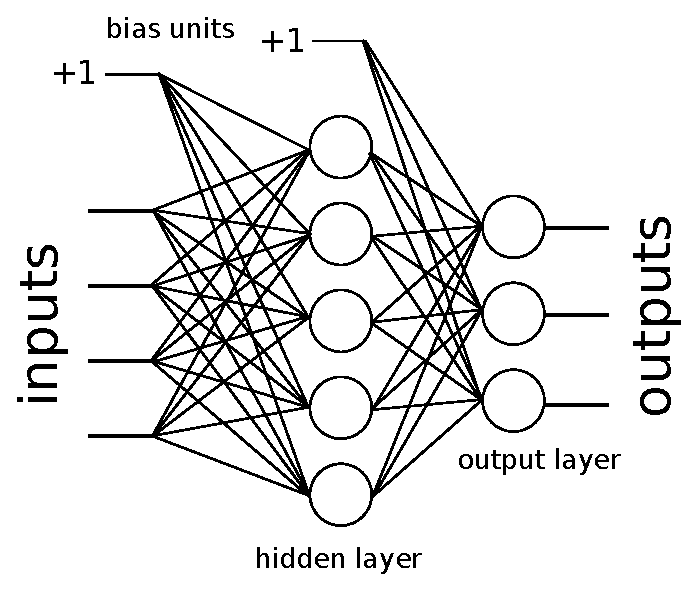
\includegraphics[width=0.5\textwidth]{diagrams/neuralnet}
\caption{A two layer feed-forward neural network}
\label{fig:neuralnet}
\end{figure}

The network topology used is shown in figure \ref{fig:neuralnet}.  It consists of two layers of neurons: the input of every neuron in the first layer (the ``hidden layer'') is connected to every input of the network, and the input of every neuron in the second layer (the ``output layer'') is connected to every output of the first layer.  Finally, the output of the network is defined by the output of the second layer.  The connections between neurons, and betwen inputs and neurons, are each associated with some weight.

Note that some textbooks describe the network as having three layers, the first being the ``input layer'': this description is avoided here, as the inputs are not processed before reaching the hidden layer, i.e., there are no neurons as such in the ``input layer''.

Notice also the two ``bias units'': if the output of each neuron is to compute some aribtrary function of the inputs, they must be able to incorporate some constant value in the function.   \citet{Aleksander1995} describe a \emph{threshold value} which serves the same purpose.  Although a separate threshold value is clearer when dealing with the theory, it will be seen later on that by treating it as a neuron or input which always gives the value 1, the implementation is simplified somewhat.

The \emph{activation} of the $j$th neuron for the $p$th training example, $a_{pj}$, is given by taking the sum for all inputs $i$ multiplied by the corresponding weight, $w_{ji}$.

\begin{equation}
a_{pj} = \sum_{(for~all~i)} w_{ji}o_{pi} + u_j
\label{eq:activation}
\end{equation}

Recalling figure \ref{fig:neuron}, the output $o_{pj}$ of a neuron is the result of some function applied to the activation (equation (\ref{eq:output})).  This function is generally a sigmoid function, and a convenient function to use is shown in equation (\ref{eq:sigmoid}).  It is convenient as its derivative is trivial to determine, and this is required later in the algorithm.  Another popular activation function is $atan(x)$.

\begin{equation}
o_{pj} = f_j(a_{pj})
\label{eq:output}
\end{equation}

\begin{equation}
f(x) = {1 \over 1 + e^{-x}}
\label{eq:sigmoid}
\end{equation}

Using the equations so far, the output of the network can be determined for a given input: first, the outputs of all the neurons in the hidden layer are calculated from the inputs to the neural network; then, the output of the final layer can be calculated from the output of the hidden layer.  It is this process that gives the structure the name ``feed-forward''.

Training the network involves presenting a training example to the network and calculating the output for it using the feed-forward process.  This will give an output, which in the case of a network with no previous training, will be much different from the expected output given by the training data.  The weights are updated as described below to correct for this error, and the training continues.  After many iterations and training examples, the output for a given output will be much closer to the expected value.

Given the $p$th training example, the amount ($\Delta_{p}w_{ji}$) that the weight which joins the $j$th neuron to its $i$th input should be adjusted by is poportional to the calculated error for the unit ($\delta_{pj}$) and a learning rate $\beta$ (equation (\ref{eq:learning})).

\begin{equation}
\Delta_pw_{ji} = \beta\delta_{pj}o_{pi}
\label{eq:learning}
\end{equation}

Calculating the error of output neurons is easy, as the training example states what the expected output is.  The error is therefore the difference between the actual output and the expected output, multiplied by the derivative of the activation function applied to the activation for that neuron (equation (\ref{eq:outputerror})).  Recall the activation function chosen is given by equation (\ref{eq:sigmoid}): its derivative is given by equation (\ref{eq:sigd}).  Note that the value $f(x)$ is the output for the neuron, and has already been calculated by the feed-forward process.

\begin{equation}
\delta_{pj} = (t_{pj} - o_{pj})f'_j(a_{pj})
\label{eq:outputerror}
\end{equation}

\begin{equation}
f'(x) = f(x)\big(1 - f(x)\big)
\label{eq:sigd}
\end{equation}

The errors for the hidden neurons are calculated by propagating the errors back from the output layer, hence the name of the algorithm.  More specifically, the error for the $j$th neuron and the $p$th training example is given by taking the sum of output all errors $k$ multiplied by the corresponding weight $w_{kj}$, all multiplied by the derivative of the activation function applied to the activation for the neuron (equation (\ref{eq:hiddenerror})).

\begin{equation}
\delta_{pj} = \left(\sum_{(for~all~k)}\delta_{pk}w_{kj}\right)f'_{j}(a_{pj})
\label{eq:hiddenerror}
\end{equation}

The described algorithm is a form of gradient descent.  It can be applied to all of the examples in succession, with this being repeated for many iterations; this is called \emph{batch gradient descent}.  As new examples arrive gradually throughout the lifetime of the agent, this project uses the alternative method of \emph{stochastic gradient descent} \citep[p. 720]{RussellNorvig}.

\subsection{Alternatives}

Backpropagation was chosen in this project due to its simplicity and ease of implementation.  Many others have made the same choice, although weaknesses such as slow convergence and a requirement to tune the learning rate are well known.

\citet{Groot1994} showed that algorithms which incorporate higher order information give both a better quality solution (reduced error) and a quicker running time.  By `higher order', the order of the derivatives used by the algorithm is being referred to.  Algorithms which used information from the second derivative of the neural network transfer function were shown to be much more effective.

An exploration of various optimisation algorithms was originally intended as part of this project; however, it turned out to be far too complex to achieve within the time frame.

\section{Proof of concept}

It was necessary to show that it is at least theoretically possible to learn ghost behaviour using neural networks.  First of all, a neural network was implemented in MATLAB; then data from a game was recorded; finally, this data was fed into the neural network implementation to determine if it could be learnt.  The various steps will be described further in the following sections.

\subsection{Neural network implementation in MATLAB}
\label{sec:matlab}

MATLAB is a mathematical programming language developed by MathWorks.  Although commercial, it is available in many organisations and institutions.  There is also an open source equivalent called Octave: this was initially used, but it lacks several useful functions needed by the project.

One of the benefits of using MATLAB to prototype the neural network is that it can perform operations on variables regardless of whether they represent scalar values or vectors.  For example, in the expression {\tt sin(x)} will return a scalar value if {\tt x} is a scalar, or a matrix of results if {\tt x} is a matrix, using each element in {\tt x} as an input.  Thus, it is convenient if the implementation of the backpropagation algorithm described in section \ref{sec:nnalgorithm} is vectorised.

The inputs to the network are represented as a column vector.  If there are $n$ inputs, there will be $n + 1$ elements in the vector, as the bias unit is added at the top.  If there are $h$ neurons in the hidden layer, the weights which govern the connections between it and the inputs are held in a $h \times (n + 1)$ matrix: for each neuron in the hidden layer, there is a weight to connect it to each of the inputs and the bias unit.  There is a similar matrix for the output layer: in the code, they are called {\tt th1} and {\tt th2} respectively, and they are initially randomly initialised.  This random initialisation is necessary for \emph{symmetery breaking}---if all weight start with the same value, they will always update by the same amount, and the network will be unable to learn anything.

The forward propagation part of the code is given by listing \ref{lst:forward}.  The variable {\tt a1} is the inputs, calculated by taking the $j$th training example and adding the bias unit.  Next {\tt a2}, the hidden layer outputs, is calculated by multiplying the inputs by the weights matrix, applying the activation function\footnote{denoted by the {\tt sig} function, the source code of which is in appendix \ref{ap:matlab}}, and adding the bias unit.  Note that due to the nature of matrix multiplication, the multiply-and-sum operation happens ``for free''.  The output layer is calculated in a similar process, but there is no need to add a bias unit.

\begin{lstlisting}[language=Matlab,label=lst:forward,caption={Forward propagation code},captionpos=b]
a1 = [1; x(j,:)'];
a2 = [1; sig(th1 * a1)];
a3 = sig(th2 * a2);
\end{lstlisting}

After the forward propagation step, backpropagation is performed (listing \ref{lst:backprop}).  The variable {\tt t} represents the target values for the output, and is a vector with a number of elements equal to the number of output nodes.  As described in section \ref{sec:nnalgorithm}, the error of the output nodes ({\tt d3}) is calculated by subtracting the actual output from the target output and multiplying by the derivative of the activation function, defined as {\tt sigd} here.  By using a vectorised implementation, one line of code can perform this function for the whole output layer.

Recall that the error in the hidden layer is given by backpropagating the error from the output layer, using the connecting weights.  The error in the hidden layer is used to calculate the adjustment needed in the weights connecting the hidden layer to the input---since the input is not connected to the bias unit, we do not need to consider it, and that is why the first column (which relates to the bias unit) of {\tt th2} is missed out.

\begin{lstlisting}[language=Matlab,label=lst:backprop,caption={Backpropagation code},captionpos=b]
d3 = (t - a3) .* sigd(a3);
d2 = (th2(:,2:end)' * d3) .* sigd(a2(2:end));
\end{lstlisting}

Now all that remains to be done is to update the weights, shown in listing \ref{lst:update}.  The weights which connect the hidden layer to the input are responsible for any errors resulting in the output of the hidden layer, and the calculated error of the hidden layer is therefore used in updating these weights.  The variable {\tt beta} is the \emph{learning rate}, and governs the rate of gradient descent.  A value of 1 has been found to work adequately.  The weights which govern the connection of the hidden layer and the output layer are updated in a similar fashion.

\begin{lstlisting}[language=Matlab,label=lst:update,caption={Weight update code},captionpos=b]
th1 = th1 + beta * d2 * a1';
th2 = th2 + beta * d3 * a2';
\end{lstlisting}

A full listing of the function described in this section, as well as the listings of the {\tt sig} and {\tt sigd} functions, can be found in appendix \ref{ap:matlab}.  This implementation was verified by ensuring that the network could learn various boolean functions from examples, such as OR, AND, and XOR.  The latter is a `hard' learning problem which can only be learned by multi-layer networks.

\subsection{Logging ghost data}

In order to prove that the concept was feasible, it was necessary to record the kind of data available in a game to the ghost controller and run the neural network implementation on it to see if it could learn the behaviour.

A class was created, namely {\tt GhostState}, to encapsulate the elements of the game state which matter to a particular ghost.  For example, inside a ghost controller class, the action of a given ghost may be dependent on the ghost's proximity to Ms~Pac-Man; or the next move to make in order to bring the ghost closer to Ms~Pac-Man; or perhaps whether the ghost is edible or not.  This information can be obtained by calling functions on the game state instance passed to the ghost and Ms~Pac-Man controller {\tt getMove} functions (described in section \ref{sec:existingagent}).

A second class, {\tt GhostLogger}, was created to handle recording this ghost information to file. The class holds a reference to an instance of {\tt GhostState} and a {\tt BufferedWriter} which handles writing to the log file.  Every tick, the {\tt log} method on the class is called, which checks if the state information held for the previous tick indicates that the ghost had to make a decision: if it did, then that state information and the decision the ghost made (which is now available, the following tick) is written to the log file as a comma-separated list of floating-point values.  The features are scaled to between 0 and 1 (approximately) by dividing the feature by the the largest value (or a value close to it).  This is necessary to ensure that the network can be trained properly.  Directions (such as the move the ghost took, or the next move away from Ms~Pac-Man) are recorded as four values corresponding to up, down, left and right: a 1 is written in the place for the indicated direction, with the rest being 0.

The ghost the logger is tracking will not make a decision every tick, so a line is only written to the file every few ticks.  Either way, the state the logger holds for the ghost is updated after checking the old state and possibly writing it out.

The {\tt GhostTeamLogger} class was also created to hold references to four instances of {\tt GhostLogger}---one for each ghost---and abstract the details away.  The class implements the {\tt GameTask} interface, which allows it to be added to a list of classes to be invoked each game tick.

The result of running the game with the {\tt GhostTeamLogger} registered as a game task is the creation of four comma-separated variable log files in the log directory, containing the decisions made by each of the four ghosts and the game state data that the decisions were based on.  This data can then be used as training examples for the neural network.

\subsection{Results}
\label{sec:conceptresults}

For each ghost, a neural network was trained using the data in the associated log file, recorded using the methods described in the previous section.  The log files were produced by playing a game against the {\tt Legacy} controller (section \ref{sec:legacy}), and the features chosen to log were fairly arbitrarily chosen as: the level time, the edible score, the number of active power pills, the number of lives remaining for Ms~Pac-Man, the amount of time left for which the ghost will stay edible (or zero if this doesn't apply), the next move away from Ms~Pac-Man and the next move towards Ms~Pac-Man (both using the Manhattan distance measure), and the distance to Ms~Pac-Man from the ghost.  These features were all scaled to be approximately between 0 and 1.  For each of the ghosts Blinky, Pinky, Inky, and Sue, there were 886, 855, 811 and 808 training examples respectively.

After training, each network was used to predict the data it was trained on, and a percentage error rate was obtained.  This was repeated ten times, and averaged for each ghost.  The results are presented in Table \ref{tab:proofconcept}, and give clear indication of learning.  Recall from Section \ref{sec:legacy} that the ghosts in the {\tt Legacy} controller choose the next move towards Ms~Pac-Man using different distance measures: Inky uses the Manhattan measure, which is the one used in the training data, so that could explain why the error rate is zero.  Also, Sue just uses random moves, which would explain why she has the highest error rate.

\begin{table}[ht]
\centering
\begin{tabular}{ll}
\toprule
Ghost & Error rate (\%) \\
\midrule
Blinky & 10.44 \\
Pinky & 24.48 \\
Inky & 0 \\
Sue & 38.61 \\
\bottomrule
\end{tabular}
\caption{Error rates for predicting ghost behaviour}
\label{tab:proofconcept}
\end{table}

Interestingly, although Blinky uses the Path distance measure and Pinky uses Euclidian (which is much closer to the available Manhattan data), it is the former which has the lower error rate.  Even so, that Inky should get a perfect score when supplied with the correct data is cause enough for the investigation in the following section.

Note that the neural networks described above could suffer from \emph{over-fitting}, that is, being particularly good at fitting the training data, but unable to generalise well to new data.  To account for this, the data used as input to the neural network when evaluating the error rate should have been different to the training data.

\subsection{Choosing the neural network features}

The analysis in section \ref{sec:sampleghosts} was the main source of information used when picking the ghost state data to use as input to the neural networks for each ghost (neural network input is often called the \emph{features}).  However, due to the similarity between the Euclidian and Manhattan distance measures, some tests were run to determine if it was really necessary to include both.  The more features a neural network has, the bigger the matrices involved and hence the longer it takes to perform operations with, so it is advantageous to keep the number of features as low as possible.

A game was recorded against the {\tt Legacy} ghost controller in a similar setup to the previous section, except that the next moves towards Ms~Pac-Man were included using all three distance measures.  The networks were then trained using some or all of this data as appropriate in a similar fashion to above.  Note that only the results for Blinky, Pinky and Inky are included, as Sue always returns random moves and bears no relation to the input.

Table \ref{tab:alldm} shows the error rates achieved after training networks for the three ghosts using data which included the next moves towards Ms~Pac-Man using all three distance measures.

\begin{table}[ht]
\centering
\begin{tabular}{ll}
\toprule
Ghost & Error rate (\%) \\
\midrule
Blinky & 7.67 \\
Pinky & 0.39 \\
Inky & 0.13 \\
\midrule
Overall average & 2.73 \\
\bottomrule
\end{tabular}
\caption{Error rates when using all distance measures}
\label{tab:alldm}
\end{table}

The training was repeated for the ghosts using the data from the same game, but with the Manhattan measure removed.  The results (Table \ref{tab:withoutmanhattan}) show the error rate for Inky---the ghost which uses the Manhattan distance measure---increasing from 0.13\% to 7.43\%; however, the overall average does not increase by a great deal.

\begin{table}[ht]
\centering
\begin{tabular}{ll}
\toprule
Ghost & Error rate (\%) \\
\midrule
Blinky & 7.04 \\
Pinky & 0.39 \\
Inky & 7.43 \\
\midrule
Overall average & 4.95 \\
\bottomrule
\end{tabular}
\caption{Error rates when the Manhattan distance measure is unavailable}
\label{tab:withoutmanhattan}
\end{table}

As a result of this, the decision was made to include only the Path and Euclid distance measures.  In the example ghosts, only {\tt Legacy} uses something other than the Path measure, and it is assumed that competition controllers are more likely to mostly only use this measure as well as it is the most useful; the Euclid distance measure is sufficiently similar to make up for the missing Manhattan measure.  At this point, the distance between Ms~Pac-Man and her closest powerpill was also added as a feature.


\subsection{Neural network implementation in Java}

As introduced in section \ref{sec:matlab}, MATLAB makes it possible to perform operations on whole matrices at once.  A method to convert this easily into Java whilst still preserving much of the terseness of the original was sought, and as a result a Matrix class was written to represent matrices in Java\footnote{There are many good matrix libraries for Java, which were considered at the time---however, it was realised that this implementation would have to be heavily optimised for the specific task, which the third-party libraries did not deal with.  See section \ref{sec:efficiency} for more details on the optimisations made.}.  The neural network code using this matrix implementation (listing \ref{lst:javanet}) is appreciably similar the MATLAB implementation, within the constraints of the Java programming language.  This similarity is useful not only as it is easier to programme, but also easier to see that it is correct if it matches the working implementation.

\begin{lstlisting}[language=Java,label=lst:javanet,caption={Java neural network code},captionpos=b]
a1 = Utilities.appendVertical(1, x.part(j, j, 1, -1).transpose());
a2 = Utilities.appendVertical(1, theta1.multiply(a1).apply(sig));
a3 = theta2.multiply(a2).apply(sig);

t = y.part(j, j, 1, -1).transpose();
d3 = t.subtract(a3).elementMultiply(a3.apply(sigd));
d2 = theta2.part(1, -1, 2, -1).transpose().multiply(d3)
        .elementMultiply(a2.part(2, -1, 1, 1).apply(sigd));

theta1 = theta1.add(d2.multiply(a1.transpose()).scale(learningRate));
theta2 = theta2.add(d3.multiply(a2.transpose()).scale(learningRate));
\end{lstlisting}

This implementation was tested with the same test data used in section \ref{sec:conceptresults}, and the algorithm achieved similar results.  It did however run appreciably slower than the MATLAB implementation, a problem addressed in section \ref{sec:efficiency}.


